\documentclass{article}

\usepackage[utf8]{inputenc}

\usepackage{graphicx}
\graphicspath{{images/}}

\renewcommand{\familydefault}{\sfdefault}
\usepackage[a4paper]{geometry}

\usepackage{listings}

\usepackage{tcolorbox}
\newtcolorbox{keypointbox}
{
    arc=0mm,
    colback=red!20,
    colframe=red!80,
    leftrule=5pt,
    toprule=0pt,
    rightrule=0pt,
    bottomrule=0pt
}

\setcounter{secnumdepth}{2}

\usepackage{amsmath}
\usepackage{amssymb}
\usepackage{bm}

\newcommand{\norm}[1]{\left\lVert#1\right\rVert}

\usepackage{hyperref}
\usepackage{cleveref}

\title{Physically Based Simulation}
\author{Alexander Schlögl}

\begin{document}
\maketitle

\tableofcontents

This is \textbf{my interpretation} of the lecture slides.
I tried to be very verbose and explain everything, all while removing irrelevant parts from the lecture.
Using this you should be able to pass the lecture easily.
\large{\textbf{However, I do not take responsibility for any bad results and will not be blamed from anyone.
This was a lot of work and I did it to save others (especially students of following semesters) from having to do this themselves.
Use this summary at your own responsibility.}}
If you have any feedback, feel free to create an issue on the \href{https://github.com/alxshine/lecture-notes}{git}.
I don't promise I will fix anything, but I will try.
\newpage

\section{Introduction to Compilers}
A compiler is a program that takes code written in a source language, which is usually a high-level language, and transforms it into a target language, often object code or machine code.
In the toolchain that transforms high level code to machine code, there also are other, compile-related programs, which may or may not work together with a compiler:
\begin{itemize}
	\item \textbf{Interpreters \& just-in-time compilers} often used for scripting languages (and Java)
	\item \textbf{Assemblers} translate the assembly language into machine code
	\item \textbf{Linkers} combine different object files into executable code
	\item \textbf{Loaders} load shared librabries (relocatable code)
	\item \textbf{Preprocessors} perform macro substitutions
	\item \textbf{Editors} are used to edit the code
	\item \textbf{Debuggers} allow step-by-step execution of the executable
	\item \textbf{Profilers} create memory and runtime profiles of the executable
	\item \textbf{Binary Inspection} allow inspection of the target code in the executable
\end{itemize}

\subsection{Language Description}
As a compiler needs to be tailored to the source and target language, describing languages is an essential part of building a compiler.
Languages are usually defined at three levels:
\begin{itemize}
	\item \textbf{Lexical level}:
		The lexical level of a language is defined by a dictionary.
		The dictionary contains a list of keywords and formats for the different data types, as well as valid variable names, usually defined using regular expressions.
	\item \textbf{Syntactical level}:
		The syntax of a language is defined by a grammar, describing valid control structures of the language.
	\item \textbf{Semantic level}:
		This describes the meaning of well-defined sentences in the language, and is often defined (in prose) in the language documentation.
\end{itemize}

\subsection{Phases of a Compiler}
A compiler operates in phases, split according to the tasks performed.
Common phases of a compiler are shown in \Cref{fig:phases}.
While the distinction between the phases is not always clear cut, keeping a degree of modularity is often beneficial.

\begin{figure}[h]
	\center
	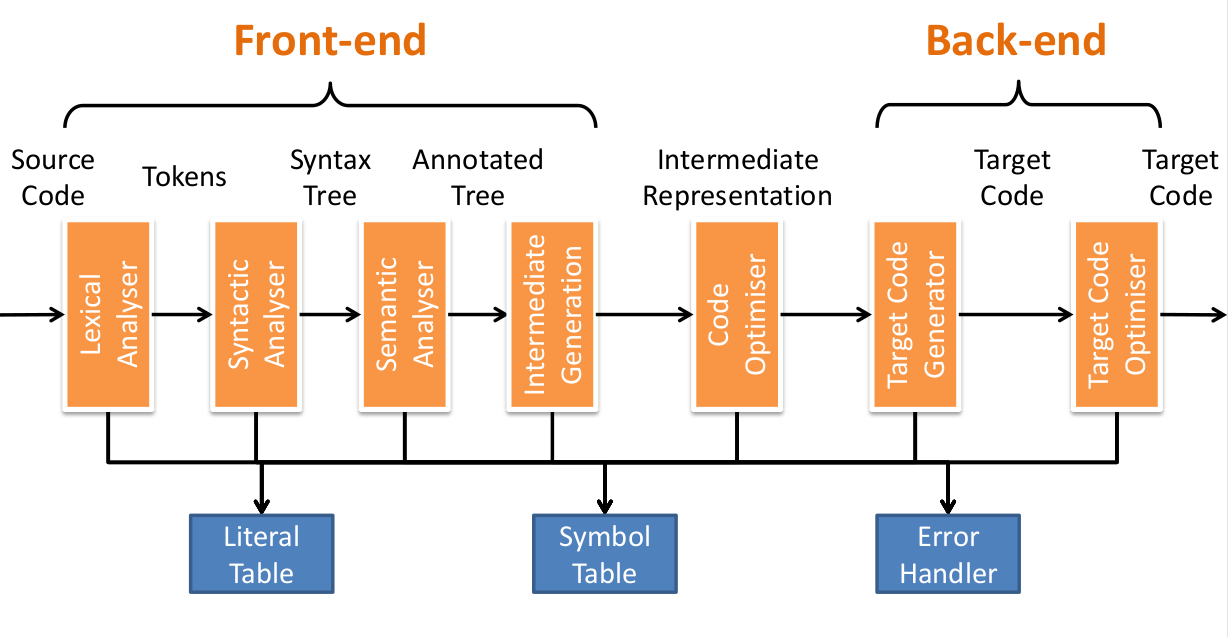
\includegraphics[width=\textwidth]{phases.png}
	\caption{The phases of a compiler}
	\label{fig:phases}
\end{figure}

\subsubsection{Lexical Analysis (Scanning)}
Scanning is the process of taking in a stream of characters and outputting a stream of tokens.
This means splitting the source code into variable names, literals, etc.
During this phase a compiler can also enter \emph{identifiers} into the \emph{symbol table} and \emph{literals} into the \emph{literal table}.

\subsubsection{Syntactic Analysis (Parsing)}
During parsing the stream of tokens is used together with a grammar to create a \emph{syntax tree} and report syntax errors to the user.

\subsubsection{Semantic Analysis}
Semantic analysis checks the meaning of the program, and annotates the syntax tree with \emph{attributes}, e.g. declarations and data types.
Some semantics can only be checked while the programming is running (think dynamically allocated arrays), so not all errors are caught here.

\subsubsection{Intermediate Code Generation}
If multiple source and target languages or platforms are going to be supported it can be very beneficial to generate an intermediate representation that is independent of platform and language.
Using an intermediate representation removes the need of creating a compiler for every combination of source and target platform.
This reduces the number of parts that need to be written from $m*n$ to $m+n$, where $m$ is the number of source platforms and $n$ is the number of target platforms.
The required for adding a new source or target platform also drops from $m$ or $n$ to $1$.

Intermediate representations also have the benefit of making optimization through multiple passes easier.
A good example of intermediate representations being used is the LLVM compiler.

\subsubsection{Code Optimizer}
The code optimizer works on the intermediate representation by applying optimizations.
An optimization is a transformation that improves performance of the code in one or more metric.
Examples are dead code eleminition, consant folding or propagation, etc.

\subsubsection{Code Generator}
During this phase the actual target code is generated.
This can be Assembler, or any other target language.
Memory management, register allocation and instruction scheduling are the main challenges here.

\subsubsection{Target Code Optimizer}
In the last phase optimizations that are target specific are done.
This includes replacing instructions with faster ones, data pre-fetching and code parallelization where possible.

\subsection{T-Diagrams}
A compiler is defined by three languages:
\begin{itemize}
	\item \textbf{Host Language}: This is the language in which the compiler itself runs.
	\item \textbf{Source Language}: This is the language of the input.
	\item \textbf{Target Language}: This is the language the compiler produces.
\end{itemize}

Any and all of these three languages can be the same.
If a compiler produces code in a language that cannot be run on the host machine (the one doing the compilation), it is called a \emph{cross-compiler}.

Compilers are often represented using T-Diagrams, with the letters denoting the different languages.
An example is shown in \Cref{fig:bootstrapping}.

\subsubsection{Bootstrapping}
In order to create a compiler for a new language, one can save some work by employing a process called \emph{bootstrapping}.
During this process, a compiler for the new language is written in the new language, as it can then make use of the many neat features that were included in the new totally not bloated language that is super awesome and will end all other programming languages (/s).
The language creators then write a quick and dirty compiler in a different language.
This compiler doesn't have to be powerful, it only needs to be able to compile the "good" compiler.
By combining the two we then get a (hopefully) correct, but inefficient compiler.
Then we can recompile the "good" compiler with the minimal one to get the final version of the compiler, which can then compile all future versions of itself (until you include new language features).
The full workflow is shown in \Cref{fig:bootstrapping}

\begin{figure}[h]
	\center
	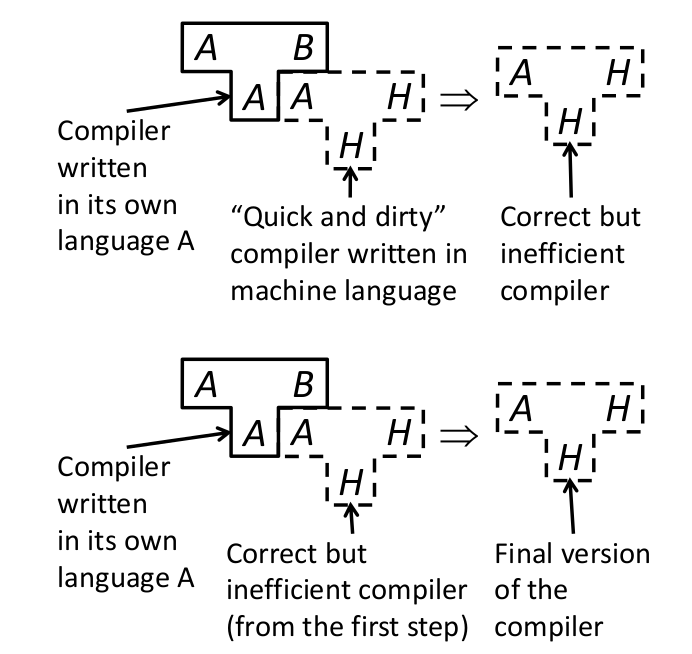
\includegraphics[width=\textwidth]{bootstrapping.png}
	\caption{The bootstrapping process in less text and more images}
	\label{fig:bootstrapping}
\end{figure}

\subsubsection{Porting}
Porting is the process of moving a compiler written it its own source language $A$ from machine $H$ to machine $K$.
In order to do this, a compiler is written in the source language $A$ with target language $K$, called a retargeted compiler.
This is then compiled with the original compiler and produces a cross-compiler.
The cross-compiler runs in language $H$ and produces language $K$ from source language $A$.
The retargeted compiler is then compiled with the cross compiler to create a compiler for language $A$ that runs in language $K$.
The entire workflow is shown in \Cref{fig:porting}

\begin{figure}[h]
	\center
	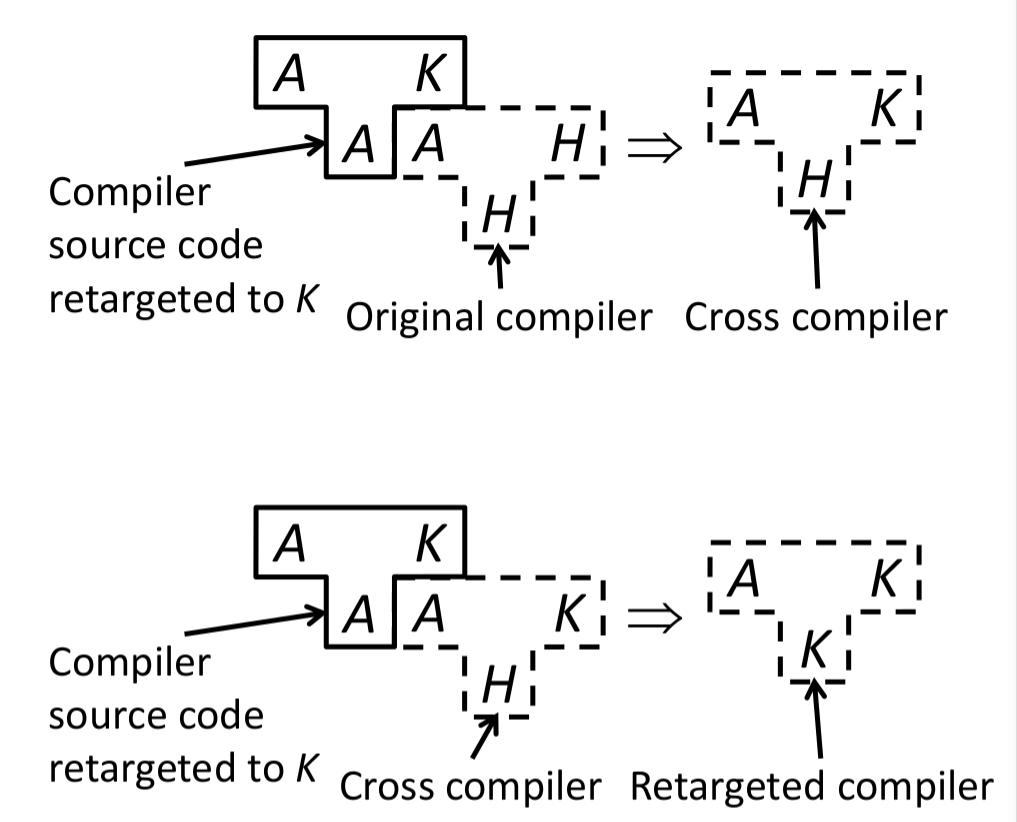
\includegraphics[width=\textwidth]{porting.png}
	\caption{Porting a compiler}
	\label{fig:porting}
\end{figure}

\subsubsection{Combining T-Diagrams}
Combining T-Diagrams is super easy and straight forward.
Just replace the language (or letter) to the left of the T-Diagram with the one on the right.
A few examples are shown in \Cref{fig:tcombining}

\begin{figure}[h]
	\center
	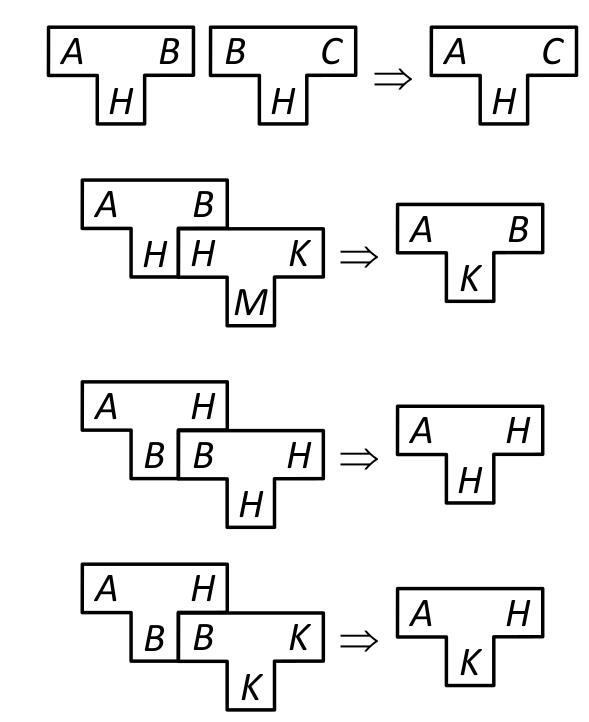
\includegraphics[width=0.8\textwidth]{tcombining.png}
	\caption{Combining T-Diagrams}
	\label{fig:tcombining}
\end{figure}

\section{Lexical Analysis (Scanning)}
During scanning we want to split a stream of characters into a stream of tokens.
The main goals are separating keywords, variables, constants, operators, etc.
We do this by creating regular expressions (regexes) for every type of token we want.
These regexes are then converted to finite automata, which we can simulate nicely.
We also want this phase of the compiler to be as efficient as possible, in order to save time for the more complex phases.

\subsection{Tokens}
Tokens in general are defined as an enumerated type, because you almost never define new keywords.
\begin{keypointbox}
	If you are using a language where you can define keywords dynamically, seek help.
\end{keypointbox}

Common token types are keywords (if, else), special symbols (+,-,*), identifiers (for variables) and numbers (int, float, ...).
These tokens can have one or more attributes, e.g. the string matched for the token (\emph{lexeme}), the numerical value for numbers, the operator for special symbols, ...
These attributes, as well as the type, are stored in a token record, which is just a simple container object or struct or whatever your language supports.
The scanner is usually controlled by the parser, which just calls it again and again, each time receiving a single token and processing it (adding it to the token table, matching grammar rules, ...).

As most of us are in computer science because we are both lazy and smart (being less dumb than the average is sufficient), we want to do as little work as possible, and because some people actually program for fun, we don't have to.
All we have to do is specify the different program tokens with regexes, and let an automatic tool build the lexical analyzer for us.

\subsection{Regular Expressions}
I will just skim regexes here because honestly, if you don't know them by now you have been cheating on all your CL exams, so why are you even reading this?
All you need to start is an alphabet $\Sigma$, and the rest works as defined by this very simple grammar:
\begin{equation*}
	E = a \in (E \cup \{\epsilon\})\ |\ E|E\ |\ EE\ |\ E^*\ |\ (E)
\end{equation*}
So can do:
\begin{itemize}
	\item letters
	\item or
	\item concatenation
	\item repitition
	\item subexpressions
\end{itemize}
as defined in this order.
The notation for regexes is quite inconsistent, but this is the bare minimum, as defined in theoretical CS.
Most tools that use regexes can do some syntactic sugar, namely $+$ for one or more repititions, $.$ for any character, $\left[a-z\right]$ for any character (works with numbers as well), $\sim$ for set negation ($\hat{ }$ for character classes) and $?$ for optional subexpressions.
With this you can create most regexes quite comfortably.

\subsubsection{Ambiguity}
Some strings may be matched by several regular expressions.
Usually the longest match is used (e.g. "forever" is not a keyword, even though it starts with "for") but sometimes even that fails.
If there is doubt, most scanners will just use the rule that comes first, but for some more granular decisions token delimiters can be needed (e.g. line end or whitespace).
However, the problem with these is that they should not be consumed but instead returned to the input stream.
This is called a lookahead character.
Usually one lookahead character is enough, but sometimes more is required.

\subsection{Deterministic Finite Automata (DFA)}
Seriously, you should know this.
For an actual implementation, you just use a switch (or a series of ifs if you have to) for the incoming character and then go to the next state accordingly.
You can also do the same thing with a transition table, and code less, but transition tables can get very large.
Then you have to decide whether you want to implement sparse matrices (or use them if you can) or write a whole bunch of stupid switches.

\subsection{Constructing DFAs from Regexes}
This works just as it did in FLAT (or FML).
You create an NFA from the regexes (usually by combining NFAs for the subexpressions), and then create a DFA from that.
There's really not much to it, but if you're still unsure, just look at the FLAT slides, or ask you friends.
\end{document}
